
\chapter{Trade policy}\label{sec:policy}

\boxx{\paragraph{Plan}
	In this chapter, we discuss countries' incentives and opportunities to influence trade flows and the welfare implications of trade policy. In particular, we provide information on how the World Trade Organization organizes the world trading system. }

\pbn
\begin{figure}[H]
	\centering
	\includegraphics[width=0.5\linewidth]{../../../pic/ie/biden-buy}
	\caption{Biden and BUY AMERICAN}
	\label{fig:biden-buy}
	\note{Foto: Jim Watson / AFP taken from \href{https://cdn.prod.www.spiegel.de/images/ba7b6473-ef75-4ed8-b63d-7417205465df_w948_r1.778_fpx40_fpy28.jpg}{www.spiegel.de}}
\end{figure}

%\pbn
\exextoc{Buy local be happy?}{
	
	In many countries, including the U.S., people tend to believe that it is better to buy at home than abroad. Discuss whether or not buying locally can be a welfare-enhancing strategy. 
	Thereto read the following excerpts:
	
	\href{https://www.buydirectusa.com/15-reasons-to-buy-american-made-products/}{www.buydirectusa.com: 15 Reasons to Buy American Made Products}
		
	\zitat{Next time you are in a store or shopping online look for the Made in USA label. The job you save by doing so could one day be your own!
	
	1. When you buy American products you support American workers. Existing jobs are saved and more employment opportunities are created.
	
	2. When you buy American Made products you support companies that are doing business in America.
	
	3. Hundreds of major American corporations are continuing to ship thousands of jobs overseas. Displacing the American worker.
	
	4. Since 2000. the United States has lost an incredible 32\% of its manufacturing jobs.
	
	4. To prevent more of our manufacturing cities all over America from being transformed from thriving communities into crime infested hellholes. What happened to Flint, MI and Camden, NJ can happen in any American city when corporations decide to move production overseas.
	
	6. China is now the number one supplier of components that are critical to the operation of US defense systems. Does this bother anyone else?
	
	7. According to the Economic Policy Institute The economy has been unable to create jobs due to America?s massive trade deficit.
	
	8. U.S. trade policies encourage businesses to relocate production of goods to other nations without penalizing them for selling those goods back to  the United States. This has resulted in millions of lost jobs for the American people.
	
	9. Since 1975, the US has imported more goods than it has exported. In 2010, the US had a deficit of \$478 billion in global trade.
	
	10. Over 30 years of trade policies such as NAFTA and CAFTA have taken jobs from the American people.
	
	11. For every \$1 billion in goods imported, the economy loses 9,000 jobs.
	
	12. No regulation or safety standards in products made overseas. Chinese-made drywall used in US homes is creating health and safety hazards.
	
	13. Moral implications of the exploitation of foreign workers and violations of child labor laws overseas.
	
	14. Environmental standards are minimal or non existent in how products are made overseas. This has an impact on everyone on the planet.
	
	15. Chinese imports accounted for more than 60\% of the recalls announced by the Consumer Product Safety Commission in 2007
	
	UPDATE
	
	16. COVID – Where did that get released from?
	
	17. When you buy products from the CCP, you are helping to fund their military which are a growing threat around the globe.
	
	18. You don’t have to swim to get the products you need.}\medskip
	
	\href{https://www.whitehouse.gov/briefing-room/statements-releases/2021/07/28/fact-sheet-biden-harris-administration-issues-proposed-buy-american-rule-advancing-the-presidents-commitment-to-ensuring-the-future-of-america-is-made-in-america-by-all-of-americas/}{Statement of The White House on July 28, 2021}
	\zitat{``The President believes that when we spend American taxpayers’ dollars, it should support American workers and businesses. In his first week in office, President Biden signed Executive Order 14005, Ensuring the Future is Made in All of America by All of America’s Workers, launching a whole-of-government initiative to strengthen the use of federal procurement to support American manufacturing.'' }\medskip
	
	 \citet[p. 16]{Dallas2002Fruits}
	\zitat{``A common myth is that it's better for
		Americans to spend their money at home
		than abroad. The best way to expose the
		fallacy in this argument is to take it to its
		logical extreme. If it'`s better for me to
		spend my money here than abroad, then
		it’s even better to buy in Texas than in
		New York, better yet to buy in Dallas than
		in Houston\dots in my own neighborhood
		\dots within my own family\dots to consume
		only what I can produce. Alone and poor.''}
}

\pbn
\section{Stylized facts on trade openness}\label{sec:Stylized facts on trade openness}
\textit{Trade Openness} refers to the outward or inward orientation of a given country's economy and touches many things including:
\enux{
	\item \textbf{Trade openness:} trade to GDP ratio
	\item \textbf{Trade policy regime:} tariff profile, border efficiency, ...
	\item \textbf{Openness to FDI:} FDI inflow to GDP, ease of doing business 
	\item \textbf{Infrastructure:} logistics performance, communications infrastructure, telephone lines, Internet
	\item \textbf{Political regime:} stability, democratic, open minded, reliable, ...
}

\pbn
%\subsubsection*{Trade: Stylized Facts}

\subsection*{Trade has grown more than proportionately with GDP}
\begin{center}
	\includegraphics[width=.71\linewidth]{../../../pic/ie/wt1_pdf}
\end{center}

´\subsection*{Export plus imports as a share of GDP}
\begin{center}
	\includegraphics[width=.71\linewidth]{../../../pic/ie/wt2_pdf}
\end{center}

\subsection*{The growth in trade is not God-given }
\begin{center}
	\includegraphics[width=.8\linewidth]{../../../pic/ie/open_historic_pdf}
\end{center}

\subsection*{The second wave of globalization was enabled by technology}
\begin{center}
	\includegraphics[width=.8\linewidth]{../../../pic/ie/tradecosts_pdf}
\end{center}

\subsection*{...and trade agreements}
\begin{center}
	\includegraphics[width=.9\linewidth]{../../../pic/ie/pta_pdf}
\end{center}

\subsection*{Regional Trade Agreements in force}
\begin{center}
	\includegraphics[width=.8\linewidth]{../../../pic/ie/rta1_pdf}
\end{center}
\note{Source: WTO}

\section{World Trade Organization}\label{sec:WTO}
\begin{minipage}{0.4\linewidth}	
	\includegraphics[width=0.9\textwidth]{../../../pic/ie/wto}
	\end{minipage}
\begin{minipage}{0.6\linewidth}	
The World Trade Organization (WTO) is an intergovernmental organization that regulates international trade and replaced in 1995 the General Agreement on Tariffs and Trade (GATT). 164 (!) countries are currently member of the WTO. 
The WTO facilitates the smooth and free flow of global trade through the administration and monitoring of a rules-based system that should among others help to make international trade (policy) more predictable. This set of rules is embodied in the WTO Agreements which are based on basic principles, that are:\bigskip
	\end{minipage}
\tv Watch: \url{https://youtu.be/3Gqq2sBWai4} \textit{The World Trade Organization (WTO) • Explained With Maps}


\boxb{\enux{
		\item  \textbf{Non-discrimination:} 
		\itex{
			\item The \textbf{Most Favoured Nation rule (MFN)} ensures non-discrimination between trading partners as it states that if a WTO member grants a country an
			advantage, it has to give such advantage to all WTO	members. Thus, a WTO member has to grant the most favorable conditions under which it allows trade in a certain product type to all other WTO members. However, there is no rule without an exceptions.\footnote{For example, a member may provide preferential 		treatment only to some countries within a free trade area or customs union, without having to extend such better treatment to all members. Another exception enables developed members to give unilateral preferential treatment to goods imported from developing countries and least-developed countries (LDCs), without having to extend such better treatment to other members.}\\
			\tv Watch: \url{https://youtu.be/Q5_Bh-Y48_E} \textit{E-Learning short videos - Most-favoured nation (MFN)}
			\item The \textbf{National Treatment Principle (NTP)} ensures non-discrimination between domestic and foreign products or services. It prohibits a member from favoring its domestic products over imported products. The NTP aims to provide equality of competitive conditions for imported products in relation to domestic products. Again, no rule without exceptions.\footnote{For example, there may be a security need to develop and purchase products domestically, or government procurement may, as is often the case, be used as a	policy tool to promote smaller business, local industry or advanced technologies, see GATT Article III:8(a). \tv Watch: \url{https://youtu.be/7o0jjajYcnk} \textit{E-Learning short videos - General Exceptions}}\\
			\tv Watch: \url{https://youtu.be/y1DW-xPGgdI} \textit{E-Learning short videos - The National Treatment Principle}
		}
		\item \textbf{Transparency:} WTO members must publish their trade regulations and changes therein. Moreover, members should respond to requests for information by other members. 
		\item \textbf{More open and predictable trade:} While the use of tariffs and quotas is not prohibited, members have committed to carry out multilateral negotiations periodically with a view to reduce the general level of trade barriers. 
}}



\pbn
\section{Dispute settlement body}
To make decisions on trade disputes between governments that are adjudicated by the organization, the WTO has established the Dispute Settlement Body (DSB). The Dispute Settlement Body is a meeting of the WTO General Council that brings together all representatives of WTO member governments, usually at the ambassador level. Any WTO member that believes another member is in violation of an obligation or WTO rule can file a complaint. The goal of the Dispute Settlement Body is then to find a solution to the dispute, including any violation. The first step is consultations between governments. If the dispute cannot be resolved through discussions, the DSB makes a decision and the offending country is ordered to correct its policies. In most cases, countries find a mutually acceptable solution to the dispute. If the offending country does not correct its policy or provide other compensation, the WTO authorizes retaliatory action by the complaining country against the offending country. The adjudication process can take some time, as can the implementation of remedies to enforce or compensate for the violation of a WTO rule. \autoref{fig:diseuro} provides an overview of the average number of active, i.e., unresolved, complaints in recent years.

\boxb{\paragraph{Up-to-date sources of information}
	\itex{
		\item \href{https://www.wto.org/english/res_e/booksp_e/dispu_settl_1995_2020_e.pdf}{Book about trade disputes from 1995 to 2020:} \bibentry{Organization2010WTO}
		\item \href{https://www.wto.org/english/tratop_e/dispu_e/dispu_e.htm}{WTO: Dispute settlement}
		\item \href{https://www.wto.org/english/tratop_e/dispu_e/dispu_maps_e.htm}{Map of disputes between WTO Members}
	}
}

\begin{center}
	\includegraphics[width=.8\linewidth]{$HOME/Dropbox/hsf/pic/ie/dischart_pdf}
	\captionof{figure}{Average annual number of active proceedings per month 1995-2018}\label{fig:dischart}\note{Annual averages are calculated on the basis of the number of active proceedings per month (January to December) over the yearly period concerned (e.g. in 2017, 39 proceedings were active per month, on average). The 2018 average is based on the number of active proceedings in January, February and March.\\
		Source: \url{www.wto.org}}\bigskip
	
\end{center}


\subsubsection*{Duration of Each Stage of Proceedings}
\begin{center}
	\includegraphics[width=.55\linewidth]{../../../pic/ie/duration_pdf}
\end{center}
Source: \cite{Johannesson2017WTO}

\subsubsection*{Most Active Countries at the WTO}
\begin{center}
	\includegraphics[width=.8\linewidth]{../../../pic/ie/userdsb_pdf}
\end{center}
Source: \citet{Reich2017effectiveness}

Referring to \citet{Reich2017effectiveness} the USA was a \textit{sinner}.
The US was also the respondent in a relatively high proportion of all issued panel reports, namely in 38\% of them (78 out 207). However, this high rate of US participation as respondent to
complaints on trade violations is still much lower than its share in suspension requests. In the years I reviewed, there were 75 complainants that prevailed over the US.  These are the cases where there
is a potential for suspension requests in case of non-compliance. Indeed, 26 of these complainants ended
up submitting suspension requests against the US.\footnote{Suspension requests are the “last station” on the long winding road of the WTO dispute settlement
	procedures and they represent the targeted member state’s unwillingness to submit to the system and to
	respect its international obligations.} That corresponds to 34.6\% of the total. In other
words, more than one third of the complainants who prevailed over the US in dispute settlement
procedures, were forced to turn to trade sanctions in their effort to obtain compliance by the US.

When China acceded to the WTO, many scholars and policy makers were very skeptical about the willingness and ability of China to comply with international trading rules.
However, the number of suspension requests that have been filed against China is zero (at the time when \cite{Reich2017effectiveness} published his study).
China’s record on compliance, at least for now and at least as measured by the number of suspension requests filed against it, seems to be perfect.

\begin{center}
	\includegraphics[width=.8\linewidth]{$HOME/Dropbox/hsf/pic/ie/diseuro_pdf}
	\captionof{figure}{Map of disputes between the European Union and the Rest of the World}\label{fig:diseuro}\note{Source: \url{www.wto.org}}\bigskip
\end{center}

\begin{center}
	\includegraphics[width=.8\linewidth]{$HOME/Dropbox/hsf/pic/ie/disus_pdf}
	\captionof{figure}{Map of disputes between the United States and the Rest of the World}\label{fig:disus}\note{Source: \url{www.wto.org}}\bigskip
\end{center}

\exextoc{God's diplomacy}{
\begin{center}
	\includegraphics[width=.3\linewidth]{../../../pic/ie/godsdiplomacy.png}
\end{center}
Watch the speech of Boris Johnson:\\
 \tv \url{https://twitter.com/mattwridley/status/1224392062587604994?s=20}\\
 What is meant with \textit{free trade is god's diplomacy}?
}

\pbn
\section{The Regional Comprehensive Economic Partnership (RCEP)}
\begin{center}
	\includegraphics[width=.9\linewidth]{../../../pic/ie/pacific}
\end{center}
The leaders of China and another 14 countries in the Asia-Pacific region have signed one of the biggest free trade deals in history, covering 2.2 billion people and 30\% of the world’s economic output.
The deal will cover nearly 28\% of global trade.

The Regional Comprehensive Economic Partnership (RCEP) was signed over a video link on November 15th after eight years of negotiations.

The deal sets the terms of trade in goods and services, cross-border investment and new rules for increasingly important areas such as electronic commerce and intellectual property. The effect on the trade of finished goods between Asian nations will be particularly marked, analysts have said.

Trade and investment flows within Asia have vastly expanded over the past decade, a trend that has accelerated amid feuding between the US and China, in which the two superpowers have imposed billions of dollars’ worth of punitive tariffs on each other’s exports.

Unlike the CPTPP -- the Comprehensive and Progressive Agreement for Trans-Pacific Partnership -- and the EU, it does not establish unified standards on labor and the environment or commit countries to open services and other vulnerable areas of their economies.

Donald Trump in 2017 pulled out of the Trans-Pacific Partnership, a deal previously envisaged as a way of curbing China’s influence.

\pbn
\section{Trade dispute between the USA and the European Union}

\tv Watch: \url{https://youtu.be/P2OhfgeAWb4} \textit{Trade Wars: How they work and who they impact}


In November 2021, President Biden has signed a deal to end tariffs on steel imports from the EU, which were imposed by his predecessor Donald Trump. But the agreement does not cover exports from the UK, putting British steelmakers at a disadvantage as is discussed in an article of the BBC, see \href{https://www.bbc.com/news/business-59113868}{UK steel makers 'left behind' as US ends trade war}.

In June 2018, the U.S. government imposed tariffs on \euro 6.4 billion worth of European steel and aluminum exports, followed by additional tariffs in January 2020 affecting approximately \euro  40 million worth of EU exports of certain steel and aluminum derivatives. The EU imposed countervailing measures on \euro 2.8 billion worth of U.S. exports to the EU in June 2018 (a similar EU response followed the second set of U.S. tariffs in 2020). The remaining countervailing measures, affecting up to \euro 3.6 billion worth of exports, were scheduled to take effect on June 1, 2021. The EU suspended these measures until December 1, 2021, to allow the parties to work together on a longer-term solution. Following today's announcement by the U.S., these measures will not be imposed.\citep{EuropeanCommission2021EU}



\begin{figure}[H]
	\begin{center}
		\includegraphics[width=.4\linewidth]{../../../pic/ie/biden-leyen}
	\end{center}
	\caption{Biden and von der Leyen on G20 leaders' summit in Rome, October 31,}
	\note{Source: \href{https://www.reuters.com/business/aerospace-defense/eu-us-end-clash-over-steel-aluminium-tariffs-work-global-deal-2021-10-31/}{REUTERS/Kevin Lamarque}}
\end{figure}

In November 2021, President Biden has signed a deal to end tariffs on steel imports from the EU, which were imposed by his predecessor Donald Trump. But the agreement does not cover exports from the UK, putting British steelmakers at a disadvantage as is discussed in an article of the BBC, see \href{https://www.bbc.com/news/business-59113868}{UK steel makers 'left behind' as US ends trade war}.

\pbn
\boxb{
	\subsection*{Boeing vs. Airbus}
Boeing has continually protested over launch aid in the form of credits to Airbus, while Airbus has argued that Boeing receives illegal subsidies through military and research contracts and tax breaks. All that yielded litigation at the WTO and a series of decisions that allowed (trade) penalties of both sides. 

For example, on 2 October 2019, the WTO approved US tariffs on \$7.5 billion worth of European goods, and officially authorized them on 14 October, despite the European Union urging for a negotiated settlement.
On 30 September 2020, however, the WTO approved the European Union's retaliatory tariffs on \$4.1 billion worth of US goods, this is in addition to the previous unimplemented sanction allowing the EU the right to impose tariffs of up to \$8.2 billion on US goods and services

This is a trade war where nobody will probably be better of in the end. For more details on this dispute, I recommend the Wikipedia entry here, see: \url{https://t1p.de/o0ph}. 


On June 15, 2021, the U.S. and the EU achieved a major breakthrough in the trade dispute between Boeing and Airbus, agreeing to end the 17-year dispute. All tariffs were suspended for five years.
}


\pbn
\section{Trump and trade}\label{sec:Trump and trade}

\subsection{Trump vs. the European Union a.k.a. Jean-Claude Juncker}
Donald J. Trump (@realDonaldTrump) March 3, 2018:
\zitat{
``The United States has an \textdollar 800 Billion Dollar Yearly Trade Deficit because of our `very stupid' trade deals and policies. Our jobs and wealth are being given to other countries that have taken advantage of us for years. They laugh at what fools our leaders have been. No more!''}\medskip

Jean-Claude Juncker, March 2, see \href{https://www.euronews.com/embed/439899}{euronews.com}:
\zitat{``So now we will also impose import tariffs. This is basically a stupid process, the fact that we have to do this. But we have to do it. We will now impose tariffs on motorcycles, Harley Davidson, on blue jeans, Levis, on Bourbon. We can also do stupid. We also have to be this stupid.''}\medskip

Donald J. Trump (@realDonaldTrump) March 3, 2018:
\zitat{
	``If the E.U. wants to further increase their already massive tariffs and barriers on U.S. companies doing business there, we will simply apply a Tax on their Cars which freely pour into the U.S. They make it impossible for our cars (and more) to sell there. Big trade imbalance!''}\medskip	

\pbn
Under president Trump, United States imposed tariffs on goods such as cars, olives, single malt whiskey, pecorino cheese, and wine. The EU, in turn, has raised tariffs on goods such as orange juice, bourbon, peanut butter, power boats, and Harley-Davidson motorcycles.\medskip

\begin{center}
	\includegraphics[width=0.5\linewidth]{$HOME/Dropbox/hsf/pic/ie/trump-juncker}
	\captionof{figure}{Juncker and Trump make a deal}\note{Source: \href{https://youtu.be/QXlxl7sLJjs}{YouTube.de}}
	\label{fig:trump-juncker}
\end{center}

On July 25, 2020, Jean-Claude Junker and Donald J. Trump met at the White House to discuss the ongoing trade dispute. They announced that the United States and the European Union would work to reduce tensions created by Trump's confrontational trade policies in the past.
%	\begin{quotation}
%		``The Geneva-based WTO has long avoided this politically fraught confrontation, which could irreparably harm the organization tasked with deciding international trade disputes. But barring any unforeseen developments, the WTO on Nov. 21 will grant requests from members including China and the European Union to determine if U.S. steel and aluminum tariffs imposed in March -- and based on national security concerns -- are legal.'' (Source: Bryce Baschuk at \url{www.bloomberg.com}\footnote{www.bloomberg.com/news/articles/2018-11-20/trump-trade-fight-heads-to-global-court-as-wto-nears-the-rubicon} on 21. November 2018)
%	\end{quotation}\bigskip

\pbn
\subsection{Trump and the WTO}
Read the following excerpt of an article by Bryce Baschuk at \url{www.bloomberg.com}\footnote{www.bloomberg.com/news/articles/2018-11-20/trump-trade-fight-heads-to-global-court-as-wto-nears-the-rubicon} on 21. November 2018:
\zitat{
	\textbf{Trump Trade Fight Heads to Global Court as WTO Nears the Rubicon}	
	{\footnotesize
		The Geneva-based WTO has long avoided this politically fraught confrontation, which could irreparably harm the organization tasked with deciding international trade disputes. But barring any unforeseen developments, the WTO on Nov. 21 will grant requests from members including China and the European Union to determine if U.S. steel and aluminum tariffs imposed in March -- and based on national security concerns -- are legal.
		
		U.S. trade officials say that the WTO has no authority to mediate national security matters and should simply issue a decision that says the matter is outside of the WTO’s remit. WTO Director-General Roberto Azevedo has gone so far as to warn countries against taking this dispute to the WTO, arguing that it instead “requires conversation at the highest political level.” The fight could end up sidelining the WTO.
		
		``\textit{If the WTO finds that Trump’s tariffs are permitted under the national security exception, it opens a gaping hole that would allow any other country the right to impose trade barriers on any product at any moment and for no particular reason other than protectionism}'' Chad Bown, a senior fellow at the Washington-based Peterson Institute for International Economics, said in an interview. ``\textit{`}.''
		
		In applying the tariffs, Washington relied on a rarely-used WTO national security exemption, which permits governments to take “any action which it considers necessary for the protection of its essential security interests.” The Trump administration has already blocked the process once, and since the rules don’t allow further preventative actions, the WTO will likely create a dispute settlement panel, which would consist of three experts. Any decision would likely be rendered in 2019 or 2020.
	}
	%Source: \url{https://www.bloomberg.com/news/articles/2018-11-20/trump-trade-fight-he
	%	ads-to-global-court-as-wto-nears-the-rubicon}
}

\pbn
\subsection{Trump and his trade war with China}\label{sec:trumpwarchina}
Donald J. Trump said in his 2016 presidential campaign:\footnote{See: \url{https://time.com/4386335/donald-trump-trade-speech-transcript/}} 

\zitat{``We allowed foreign countries to subsidize their goods, devalue their currencies, violate their agreements and cheat in every way imaginable, and our politicians did nothing about it. Trillions of our dollars and millions of our jobs flowed overseas as a result. I have visited cities and towns across this country where one-third or even half of manufacturing jobs have been wiped out in the last 20 years. Today, we import nearly \$800 billion more in goods than we export. We can’t continue to do that. This is not some natural disaster, it’s a political and politician-made disaster. Very simple. And it can be corrected and we can correct it fast when we have people with the right thinking. Right up here.
	[\dots] 
	To understand why trade reform creates jobs, and it creates a lot of them, we need to understand how all nations grow and prosper. Massive trade deficits subtract directly from our gross domestic product. From 1947 to 2001, a span of over five decades, our inflation-adjusted Gross Domestic Product grew at a rate of 3.5 percent. However, since 2002, the year after we fully opened our markets to Chinese imports, the GDP growth rate has been cut in half.
	[\dots]
	A Trump administration will change our failed trade policies, and I mean quickly.''}

I don't want to go into details about the trade disputes of China and USA. A nice and continually revised overview is offered by Wikipedia, see \url{https://t1p.de/y216}.

The following charts show the trade surplus/deficit (exports minus imports) for the USA, China, Russia, and Germany. The data were downloaded on 15th of June 2022 from \href{https://tradingeconomics.com/united-states/balance-of-trade}{https://tradingeconomics.com}.

\begin{center}
	\includegraphics[width=0.7\linewidth]{../../../pic/ie/us22}\captionof{figure}{United States: Balance of Trade}
	\includegraphics[width=0.7\linewidth]{../../../pic/ie/chi22}\captionof{figure}{China: Balance of Trade}
	\includegraphics[width=0.7\linewidth]{../../../pic/ie/rus22}\captionof{figure}{Russia: Balance of Trade}
	\includegraphics[width=0.7\linewidth]{../../../pic/ie/ger22}\captionof{figure}{Germany: Balance of Trade}
\end{center}

The charts indicate that Trump was not successful in reducing the trade deficit. 
Overall, it seems to be the case that trade wars are not that easy to win with respect to trade deficit and that it is not that easy to create jobs and boost the economy with starting trade disputes. 
For those who are interested: Here is a well researched article about that topic by Ryan Hass and Abraham Denmark, entitled \textit{More pain than gain: How the US-China trade war hurt America}. see: \url{https://t1p.de/2xob}.



\pbn
\exextoc{Trump complains about the WTO}{
	\enxx{a)}{\item In an interview Donald Trump said \zitat{[\dots] I called NAFTA the second-worst trade deal ever made. I would say the WTO was the single worst trade deal ever made.
			
			And if they don’t shape up, I would withdraw from the WTO. We rarely won a lawsuit except for the last year. You know, in the last year, we’re starting to win a lot. You know why? Because they know if we don’t, I’m out of there. I’ll take them out.\footnote{Source: https://www.bloomberg.com/news/articles/2018-08-31/president-donald-trump-interviewed-by-bloomberg-news-transcript}}
		%	Consider the following news excerpt:
		%\begin{center}
		%	\includegraphics[width=.75\linewidth]{pic/uswithdraw}
		%	\captionof{figure}{Trump threatens to withdraw from World Trade Organization}\label{fig:uswithdraw}\note{Source: \url{https://www.cnbc.com/2018/08/30/trump-threatens-to-withdraw-from-world-trade-organization.html}}\bigskip
		%\end{center}
		Discuss the legal constitution of the WTO and whether Donald Trump is right when he claims that other countries treat the United States unfair.\bigskip
		
		\item WTO members are not permitted to increase import tariffs without justification. An exception to this rule, however, is given when the `national security' of a nation is at risk. On this basis (which has been challenged within the WTO by several nations, including Canada), U.S. President Trump has issued executive orders imposing import tariffs on steel and aluminum imports for a set of different countries.\medskip
		
		Discuss whether this behavior can be considered as fair.
}}

\pbn
\solx{Trump complains about the WTO}{
	\enxx{a)}{\item  Trump's claims are difficult to assess because it is unclear what he means by fairness or how to define fairness in trade relations in general. 

		When referencing WTO rules, U.S. policy is far from a model of fairness to others, as too many countries have sued the U.S. for its discriminatory policies. Although he is wrong in his claim that the U.S. has "rarely won a lawsuit, with the exception of last year" (the U.S. win rate is similar to the average win rate), the U.S. is the country that has sued other members more often than any other country. For a more in-depth discussion, I recommend the article \href{http://theconversation.com/why-trumps-wrong-about-wto-treating-us-unfairly-102562}{Why Trump's wrong about WTO treating US unfairly}
		\item Imposing and increasing tariffs based on the exception rule could irreparably damage the WTO's authority to adjudicate trade disputes. This is because U.S. trade representatives contend that the WTO does not have the authority to mediate national security issues and should simply issue a ruling that the matter is not within the WTO's jurisdiction. This argument puts a gun to the WTO's head. If the WTO's Dispute Settlement Body follows this line of reasoning, any country could easily impose tariffs in the future, citing \textit{national security}, without the WTO being able to judge whether or not the issue is truly one of national security. This reminds (me) of the Mexican standoff, i.e., a confrontation between three or more parties in which there is no strategy that allows one party to win.
	}
}

\pbn
\section{Arguments for trade restrictions}\label{sec:Arguments for trade restrictions}
There are hundreds of plausible arguments to restrict international trade. Here is a in-comprehensive list of often stated arguments. Each one is a topic of its own and it needs further investigation whether these arguments are really valid arguments for restricting trade.

\subsubsection*{The desire to reduce domestic unemployment}
As we learned in the previous sections, the domestic production is the result of the world market price in the long-run. However, in the short run this means that production factors need to reallocate from one sector to the other. So far, we assumed that this reallocation happens without any frictions. Thus, we just moved along the PPF curve. In reality the transformation process is costly because the people loose their jobs without finding a job in another sector instantaneously without any costs. In reality a transformation process comes along with costs such as social costs and search and matching costs. Thus, it can be a rational strategy to decrease the reallocation/transformation pressure in order to organize the reallocation of productions factors properly holding the external negative effects of transformation low. Nevertheless, we should not forget that (in the long run) reallocation of production factors and the adaption of new technologies is basically one of the most important sources of welfare growth, if not the only source.

\subsubsection*{The key enabling technology argument}
If domestic industries are fostered, there might be technological spillovers to other industries in the country. As the government internalizes these spillovers, they have an incentive to protect and support these key to growth industries and technologies, respectively.

\pbn

\subsubsection*{The need to counteract dumping in international trade}
Selling goods in a foreign market below the price charged domestically can be called dumping. This sort of price competition is harmful when foreign producers hamper competition and discourage innovation and upgrading. For example, predatory dumping can give arguments for anti-dumping policy interventions. Predatory dumping is a type of anti-competitive behavior in which a foreign company prices its products below market value in an attempt to drive out domestic competition. This may lead to conditions where the company has a monopoly in a certain product or industry in the targeted market with bad implications for social welfare. 



\subsubsection*{The government revenue argument}
Government can finance their budget by raising tariffs.

\subsubsection*{The national defense argument}
National defense is an obviously legitimate goal for any sovereign government and hence, domestic industries that supply goods and services that are important for a potential military emergency should have a special protection.

\subsubsection*{The wish to decrease the national balance of payments deficit}
Countries that have a large trade deficit wish---for whatever reason (see \autoref{sec:balance-of-payments})---to increase import restrictions in order to decrease the export deficit.

\subsubsection*{The income redistribution argument}
As we have learned, trade generates winners and losers and hence is a source for the distribution of wealth. Government can use this knowledge to redistribute income or decrease income inequality. However, it is almost certain that this politic is not the most efficient and best way to achieve the said goals because we have also learned that trade is beneficial for a country as a whole.

\subsubsection*{The infant industry argument}

\begin{figure}[h]
	\begin{center}
		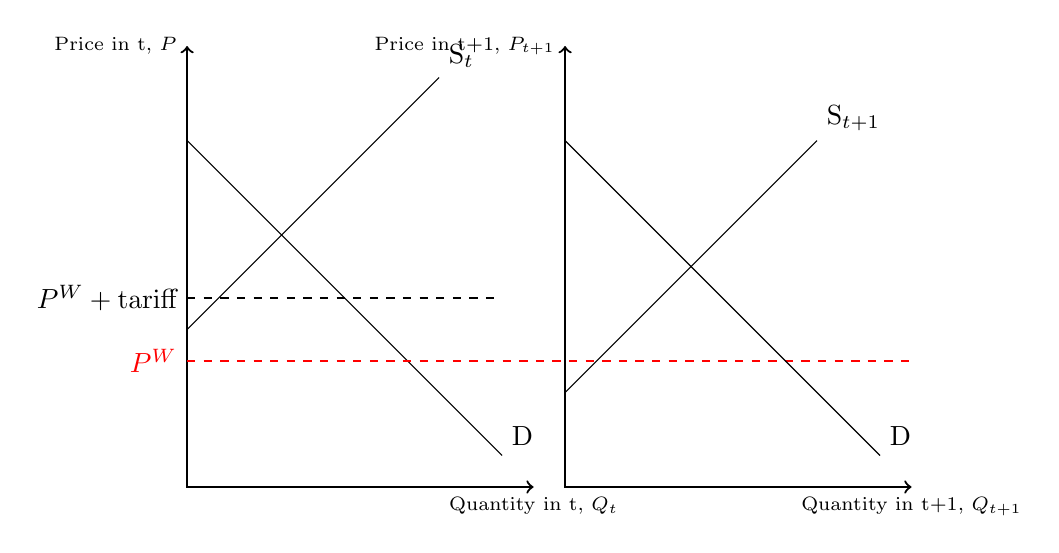
\begin{tikzpicture}[xscale=.4,yscale=.4]
			%				\draw [color=gray!50,opacity=0.5]  [step=10mm] (0,0) grid (10,10);
			%HOME	
			\draw[thick,<->] (0,14) node[left,font=\scriptsize]{Price in t, $P$}--(0,0)--(11,0) node[below,font=\scriptsize]{Quantity in t, $Q_{t}$}; 
			\draw (0,11) -- (10,1) node[above right] {D};
			\draw (0,5) -- (8,13) node[above right] {S$_{t}$};
			\draw[dashed,thick,red] (0,4) node[left]{$P^W$} -- (23,4)  ;
			\draw[dashed,thick] (0,6) node[left]{$P^W+\textnormal{tariff}$} -- (10,6)  ;
			%	\path[fill=yellow,opacity=0.3]	(0,5) -- (3,8) -- (0,8);
			%	\path[fill=blue,opacity=0.3]	(0,8) -- (3,8) -- (0,11);
			
			%FOREIGN
			%	\draw [color=gray!50,opacity=0.5]  [step=10mm] (12,0) grid (22,10);
			\draw[thick,<->] (12,14) node[left,font=\scriptsize]{Price in t+1, $P_{t+1}$}--(12,0)--(23,0) node[below, font=\scriptsize]{Quantity in t+1, $Q_{t+1}$}; 
			\draw (12,11) -- (22,1) node[above right] {D};
			\draw (12,3) -- (20,11) node[above right] {S$_{t+1}$};
			%	\draw[dashed] (12,4) node[left]{$P^H$} -- (16,4)  ;
			%	\fill[fill=yellow,opacity=0.3] (12,0) -- (16,4) -- (12,4) ;
			%	\fill[fill=blue,opacity=0.3] (12,4) -- (16,4) -- (12,8) ;
		\end{tikzpicture}
		\caption{The infant industry argument}\label{fig:infant}
	\end{center}		
\end{figure}

The basic idea is that no economic activities will happen in industries in which there are no possibilities to make positive profits because competition from abroad is currently to strong. A finite protection from international competition can make firms to grow and become more productive so that they can face foreign competition after the protection is abolished. The core of the argument is that infant industries do not have economies of scale like competitors from abroad and, hence, need to be protected until they can attain similar economies of scale.

\autoref{fig:infant} provides a schematic for understanding the infant industry argument. In the left panel you see that the domestic supply curve lies above the world market price, $P^W$. Thus, the domestic industry is not competitive enough to produce at costs lower than the world market price. A tariff in time $t$ would protect the domestic market so that some firms start to produce and sell their goods at home. The hope of the government now is that the firms become more productive over time and in turn their supply curve shifts downwards. The downward shifted supply curve in time $t+1$ is shown in the right panel. Here, the government can remove the tariff without crowding out the domestic production. 


\pbn
	\exextoc{Arguments for trade restrictions}{Explain briefly (2-3 sentences) the infant industry argument.}


\solx{Arguments for trade restrictions}{A finite protection from international competition can make firms to grow and become more productive so that they can face foreign competition after the protection is abolished. The core of the argument is that infant industries do not have economies of scale like competitors from abroad and, hence, need to be protected until they can attain similar economies of scale.}


\pbn
\section{Gains from trade}\label{sec:gains from trade}
\autoref{fig:gft1} and \autoref{fig:gft2} contain domestic supply and demand curves. In autarky with no possibilities to trade, supply and demand must meet. Under free trade and a given world market price, $P^W$, countries can trade with each other. This has implications for the producer surplus (yellow area) and the consumer surplus (blue area), as shown in the figures. The area of the triangles a and b as denoted in \autoref{fig:gft2} represents the welfare gain from free trade that can be achieved given the world market price, $P^W$.

\begin{centering}
	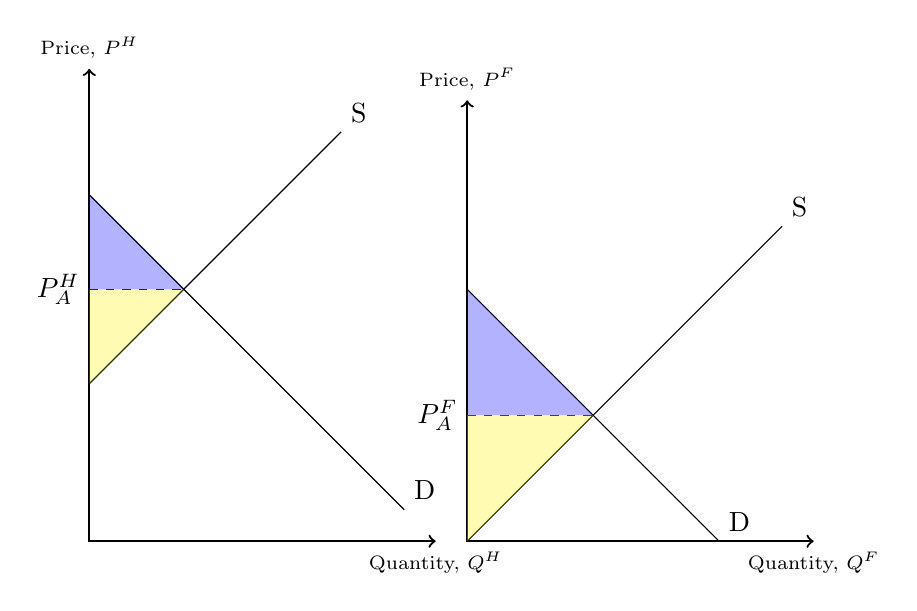
\begin{tikzpicture}[xscale=.4,yscale=.4]
		%				\draw [color=gray!50,opacity=0.5]  [step=10mm] (0,0) grid (10,10);
		%HOME	
		\draw[thick,<->] (0,15) node[above,font=\scriptsize]{Price, $P^H$}--(0,0)--(11,0) node[below,font=\scriptsize]{Quantity, $Q^H$}; 
		\draw (0,11) -- (10,1) node[above right] {D};
		\draw (0,5) -- (8,13) node[above right] {S};
		\draw[dashed] (0,8) node[left]{$P^H_A$} -- (3,8)  ;
		\path[fill=yellow,opacity=0.3]	(0,5) -- (3,8) -- (0,8);
		\path[fill=blue,opacity=0.3]	(0,8) -- (3,8) -- (0,11);
		
		%FOREIGN
		%	\draw [color=gray!50,opacity=0.5]  [step=10mm] (12,0) grid (22,10);
		\draw[thick,<->] (12,14) node[above,font=\scriptsize]{Price, $P^F$}--(12,0)--(23,0) node[below, font=\scriptsize]{Quantity, $Q^F$}; 
		\draw (12,8) -- (20,0) node[above right] {D};
		\draw (12,0) -- (22,10) node[above right] {S};
		\draw[dashed] (12,4) node[left]{$P^F_A$} -- (16,4)  ;
		\fill[fill=yellow,opacity=0.3] (12,0) -- (16,4) -- (12,4) ;
		\fill[fill=blue,opacity=0.3] (12,4) -- (16,4) -- (12,8) ;
	\end{tikzpicture}
	\captionof{figure}{Two countries in autarky}\label{fig:gft1}\end{centering}	



\begin{centering}
	\begin{tikzpicture}[xscale=.4,yscale=.4]
		%			\draw [color=gray!50,opacity=0.5]  [step=10mm] (0,0) grid (10,10);
		%HOME	
		\draw[thick,<->] (0,15) node[above,font=\scriptsize]{Price, $P^H$}--(0,0)--(11,0) node[below,font=\scriptsize]{Quantity, $Q^H$}; 
		\draw (0,11) -- (10,1) node[above right] {D};
		\draw (0,5) -- (8,13) node[above right] {S};
		\draw[dashed] (0,8) node[left]{$P^H_A$} -- (3,8)  ;
		\draw[thick, red] (0,6) node[left]{$P^W$} -- (22,6)  ;
		\path[fill=yellow,opacity=0.3]	(0,5) -- (1,6) -- (0,6);
		\path[fill=blue,opacity=0.3]	(0,6) -- (5,6) -- (0,11);
		\draw[{Latex[length=3mm]}-{Latex[length=3mm]}, thick] (1,0) node[below right=4mm]{Import} -- (5,0)  ;
		\draw[dashed] (1,-.5)  -- (1,6)  ;
		\draw[dashed] (5,-.5)  -- (5,6)  ;
		\draw (3,7) node {a};
		%		\fill[fill=black!30,opacity=0.2] (D) -- (A) -- (B) -- (C) -- cycle;
		
		%FOREIGN
		%\draw [color=gray!50,opacity=0.5]  [step=10mm] (12,0) grid (22,10);
		\draw[thick,<->] (12,14) node[above,font=\scriptsize]{Price, $P^F$}--(12,0)--(23,0) node[below, font=\scriptsize]{Quantity, $Q^F$}; 
		\draw (12,8) -- (20,0) node[above right] {D};
		\draw (12,0) -- (22,10) node[above right] {S};
		\draw[dashed] (12,4) node[left]{$P^H_F$} -- (16,4)  ;
		\fill[fill=yellow,opacity=0.3] (12,0) -- (18,6) -- (12,6) ;
		\fill[fill=blue,opacity=0.3] (12,6) -- (14,6) -- (12,8) ;
		\draw[{Latex[length=3mm]}-{Latex[length=3mm]}, thick] (14,0) node[below right=4mm]{Export} -- (18,0)  ;
		\draw[dashed] (14,-.5)  -- (14,6)  ;
		\draw[dashed] (18,-.5)  -- (18,6)  ;
		\draw (16,5) node {b};
		%	\draw[dashed] (Fx) node[below] {$\left(\frac{w}{r}\right)^H_{\textnormal{autarky}}$} -- (F) -- (0,3) node[left] {$\left(\frac{p_y}{p_x}\right)^H_{\textnormal{autarky}}$};
	\end{tikzpicture}
	\captionof{figure}{Two countries that trade with each other}\label{fig:gft2}\end{centering}	

\pbn
\section{Tariffs and quotas in small open economies}
\subsubsection{Tariff}
\autoref{fig:t1} can teach us a lot about the impact of a tariff $t$ on trade and welfare. A tariff raises the domestic price of imported goods. If we assume that the imposition or change of a country's tariff has no effect on the world price, we consider what is called a small open economy, which is so small that the country's consumption and production decisions do not affect the world price. In other words, the country takes the world price for granted because its import demand does not change the world price.


In autarky, the economy represented in \autoref{fig:t1} would consume 5 units at price $P^A$, and total welfare would be represented by areas $a+b_2+b_1$.
Under free trade without tariffs, the country imports 8 units and consumes 9 units at the price of $P^W$. The consumer surplus corresponds to areas $a+b_2+d_1+c+d_2$ and the producer surplus corresponds to area $b_1$. 
After the introduction of tariff $t$, the consumer surplus is equal to area $a$ and the producer surplus is equal to area $b_1+b_2$. Thus, consumer surplus has decreased while producer surplus has increased. The area $c$ is equal to the government's revenue. It represents the portion of the consumer welfare loss that is transferred to the government. Overall, welfare has decreased. The welfare loss is equal to the areas of the two triangles $d_1$ and $d_2$. These triangles represent what is called the \textit{deadweight loss} due to the tariff.   
Specifically, triangle $d_1$ represents the reduction in imports that is replaced by domestic production, and triangle $d_2$ represents the loss in consumption due to a reduction in imports and a reduction in domestic consumption.

\begin{centering}
	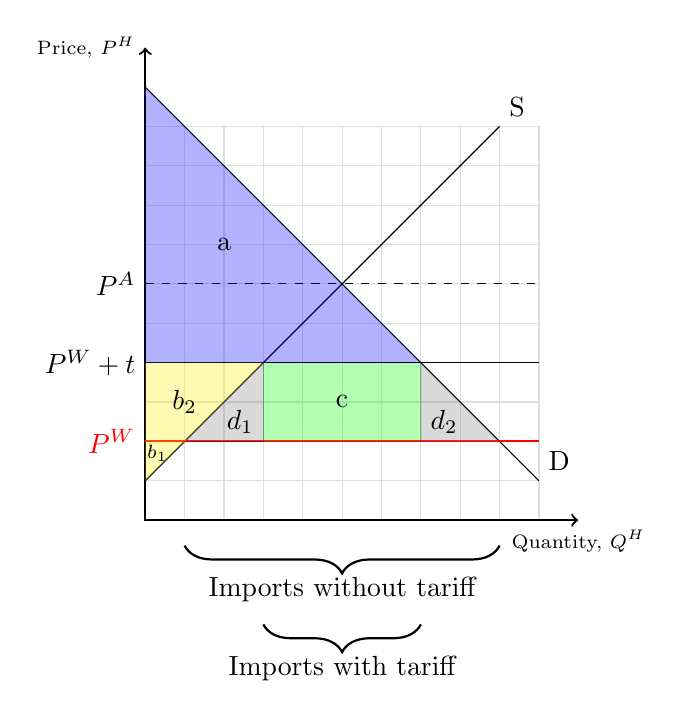
\begin{tikzpicture}[xscale=.5,yscale=.5]
		\draw [color=gray!50,opacity=0.5]  [step=10mm] (0,0) grid (10,10);
		%HOME	
		\draw[thick,<->] (0,12) node[left,font=\scriptsize]{Price, $P^H$}--(0,0)--(11,0) node[below,font=\scriptsize]{Quantity, $Q^H$}; 
		\draw (0,11) -- (10,1) node[above right] {D};
		\draw (0,1) -- (9,10) node[above right] {S};
		%	\draw[dashed] (0,8) node[left]{$P^H_A$} -- (3,8)  ;
		\draw (0,4) node[left]{$P^W+t$} -- (10,4)  ;
		\draw[dashed] (0,6) node[left]{$P^A$} -- (10,6)  ;
		\draw[thick, red] (0,2) node[left]{$P^W$} -- (10,2)  ;
		\path[fill=green,opacity=0.3]	(3,2) -- (3,4) -- (7,4) -- (7,2);
		\fill[fill=yellow,opacity=0.3] (0,1) -- (3,4) -- (0,4) ;
		\fill[fill=blue,opacity=0.3] (0,4) -- (7,4) -- (0,11) ;
		\draw[fill=gray,opacity=0.3] (1,2) -- (3,2) -- (3,4)  ;
		\draw[fill=gray,opacity=0.3] (7,2) -- (7,4) -- (9,2)  ;
		%	\draw[{Latex[length=3mm]}-{Latex[length=3mm]}, thick] (1,0) node[below right=4mm]{Import} -- (5,0)  ;
		%	\draw[dashed] (1,-.5)  -- (1,6)  ;
		%	\draw[dashed] (5,-.5)  -- (5,6)  ;
		\draw (5,3) node {c};
		\draw (1,3) node {$b_2$};
		\draw (-.2,1.7) node[right,font=\scriptsize] {$b_1$};
		%	\draw (2,7) node {a};
		\draw (2,7) node {a};
		\draw (3,2.5) node[left] {$d_1$};
		\draw (7,2.5)  node[right] {$d_2$};
		\draw [thick,decoration={brace,mirror,amplitude=10pt,raise=-5pt},decorate] (3,-3) -- (7,-3) node[midway,below,yshift=-.1cm] {Imports with tariff};
		\draw [thick,decoration={brace,mirror,amplitude=10pt,raise=-5pt},decorate] (1,-1) -- (9,-1) node[midway,below,yshift=-.1cm] {Imports without tariff};
	\end{tikzpicture}
	\captionof{figure}{Tariff in a small open economy}\label{fig:t1}\end{centering}	

\heux{The implications of a tariff in a small economy}{
	While a tariff protects domestic producers and increases their surplus, it reduces the surplus of consumers and leads to a deadweight loss of revenue. Overall, a tariff leads to a reduction in a country's welfare.}


\subsubsection{Import quota}
\begin{minipage}{0.55\linewidth}	
	A trade restriction that sets a physical limit on the quantity of a good to be imported is called an import quota. It gives government officials more power and control than a tariff because they can strictly limit the quantity of goods traded and have the administrative authority to grant (or sell) import licenses to certain foreign exporters. 
	
	\autoref{fig:importquotasmall} shows the impact of an import quota that allows an import quantity of 4 units. In this scenario, 7 units are consumed, four of which are imported. The price at which all seven units are consumed is $P*$. This is somewhat surprising because the world price $P^W$ is less than $P^*$. The reason is that all firms that are allowed to sell their products do so at the highest possible price, i.e., $P^*$.  As above, the blue area is the consumer surplus and the yellow area is the producer surplus. The gray area is the loss in value due to the import rate. The rectangle $c$ is only part of this loss, since we assume that the government does not sell the licenses to the best bidding exporting firm
\end{minipage}
\begin{minipage}{0.45\linewidth}	
	
	\begin{centering}
		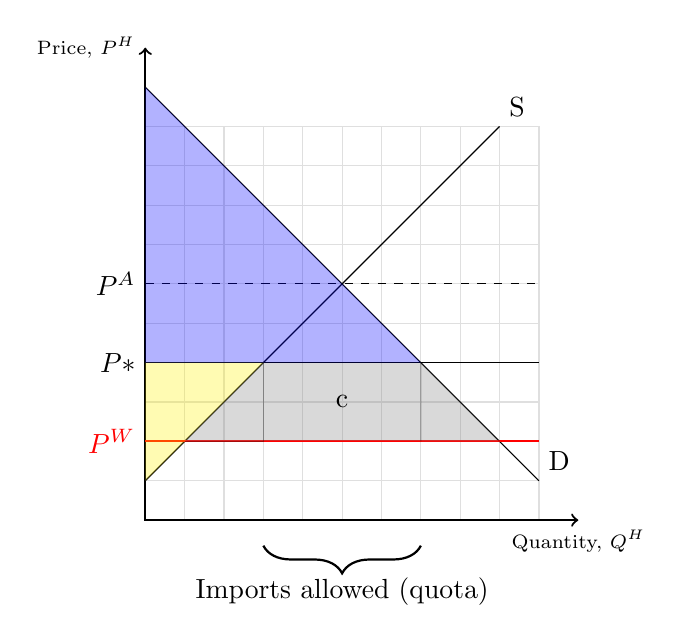
\begin{tikzpicture}[xscale=.5,yscale=.5]
			\draw [color=gray!50,opacity=0.5]  [step=10mm] (0,0) grid (10,10);
			%HOME	
			\draw[thick,<->] (0,12) node[left,font=\scriptsize]{Price, $P^H$}--(0,0)--(11,0) node[below,font=\scriptsize]{Quantity, $Q^H$}; 
			\draw (0,11) -- (10,1) node[above right] {D};
			\draw (0,1) -- (9,10) node[above right] {S};
			%		\draw[dashed] (3,0) -- (10,7) node[above right] {S};
			%	\draw[dashed] (0,8) node[left]{$P^H_A$} -- (3,8)  ;
			\draw (0,4) node[left]{$P*$} -- (10,4)  ;
			\draw[dashed] (0,6) node[left]{$P^A$} -- (10,6)  ;
			\draw[thick, red] (0,2) node[left]{$P^W$} -- (10,2)  ;
			\path[fill=gray,opacity=0.3]	(3,2) -- (3,4) -- (7,4) -- (7,2);
			\fill[fill=yellow,opacity=0.3] (0,1) -- (3,4) -- (0,4) ;
			\fill[fill=blue,opacity=0.3] (0,4) -- (7,4) -- (0,11) ;
			\draw[fill=gray,opacity=0.3] (1,2) -- (3,2) -- (3,4)  ;
			\draw[fill=gray,opacity=0.3] (7,2) -- (7,4) -- (9,2)  ;
			%	\draw[{Latex[length=3mm]}-{Latex[length=3mm]}, thick] (1,0) node[below right=4mm]{Import} -- (5,0)  ;
			%	\draw[dashed] (1,-.5)  -- (1,6)  ;
			%	\draw[dashed] (5,-.5)  -- (5,6)  ;
			\draw (5,3) node {c};
			%	\draw (1,3) node {$b_2$};
			%	\draw (-.2,1.7) node[right,font=\scriptsize] {$b_1$};
			%	%	\draw (2,7) node {a};
			%	\draw (2,7) node {a};
			%	\draw (3,2.5) node[left] {$d_1$};
			%	\draw (7,2.5)  node[right] {$d_2$};
			%	\draw [thick,decoration={brace,mirror,amplitude=10pt,raise=-5pt},decorate] (3,-3) -- (7,-3) node[midway,below,yshift=-.1cm] {Import quota};
			\draw [thick,decoration={brace,mirror,amplitude=10pt,raise=-5pt},decorate] (3,-1) -- (7,-1) node[midway,below,yshift=-.1cm] {Imports allowed (quota)};
		\end{tikzpicture}
		\captionof{figure}{Tariff in a small open economy}\label{fig:importquotasmall}\end{centering}	
\end{minipage}
%\heux{Trade restrictions are harmful}{
%For small open economies any form of trade restrictions creates inefficiencies and lowers the wealth of both the importing and the exporting country. However, producers 
%}



\pbn
\section{Tariffs in large open economies}
So far, we have assumed that the country of interest is small and takes the world market price as given. However, large countries' demand for imported goods can have an impact on world prices. If this is the case, we can show that a tariff can actually improve a country's welfare. \autoref{fig:tarlarg} illustrates the effects of a tariff on welfare, prices, and trade. In particular, we show the impact of a small tariff of 6 euros per bicycle.

Under free trade, the market for bicycle imports is cleared at a price of \euro 300 and the country imports one million bicycles. 

Now, if a tariff of \euro 6 per bicycle is imposed, the tariff drives a wedge between the price foreign exporters receive and the price domestic buyers of imports pay. That is, it becomes more expensive for domestic buyers to purchase imported bicycles. This, in turn, leads to an immediate drop in domestic demand for bicycles and pushes the world market price for bicycles to 297 euros. Given the new world market price for bicycles, the domestic price for imported bicycles is 303 euros (297+6).  

The consumer surplus is now represented by the blue area and the producer surplus by the yellow area. The green area represents the tariff revenue collected by the government. The two gray triangles, in turn, show the tariff-related deadweight losses. Compared to the free trade scenario, the country gains rectangle $c_2$. If the revenue in this area is greater than the deadweight loss, the country has improved its overall welfare by imposing a tariff. 

Let us calculate whether this is the case here:
\itex{
	\item Area  $c_2$: \[(1.58 \textnormal{ million bikes} - 0.62 \textnormal{ million bikes})\cdot (\euro 300-\euro 297)=\euro 2.88 \textnormal{ million}\]
	\item Deadweight loss:\label{dwl_loe} \[
	\underbrace{\frac{(0.62 \textnormal{ mio b.}-0.6 \textnormal{ mio b.})\cdot (\euro 303 - \euro 300)}{2}}_{\text{left triangle}} + \underbrace{\frac{(1.6 \textnormal{ mio b.}-1.58 \textnormal{ mio b.})\cdot (\euro 303 - \euro 300)}{2}}_{\text{right triangle}}=\euro 0.06 \textnormal{ million}
	\]
	\item Indeed, the net gain is 2.82 million Euros. Thus, a small tarrif can increase the welfare of a country. 
	
	
	
	\begin{centering}
		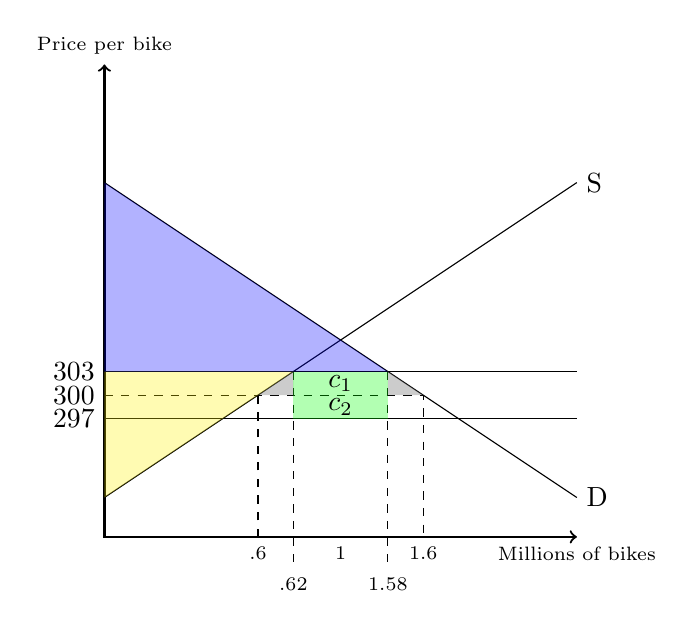
\begin{tikzpicture}[xscale=3,yscale=1]
			%				\draw [color=gray!50,opacity=0.7]  [step=5mm] (0,0) grid (2,6);
			%HOME	
			\draw[thick,<->] (0,6) node[above,font=\scriptsize]{Price per bike}--(0,0)--(2,0) node[below,font=\scriptsize]{Millions of bikes}; 
			\draw (0,.5) -- (2,4.5) node[right] {S};
			\draw (0,4.5) -- (2,.5) node[right] {D};
			\draw[] (0,2.1) node[left]{303} -- (2,2.1)  ;
			\draw[dashed] (0,1.8) node[left]{300} -- (1.35,1.8) -- (1.35,0) node[below,font=\scriptsize]{1.6} ;
			\draw[dashed] (.65,0) node[below,font=\scriptsize]{.6} -- (.65,1.8) ;
			\draw[dashed] (1,0) node[below,font=\scriptsize]{1}  ;
			\draw[] (0,1.5) node[left]{297} -- (2,1.5)  ;
			%	\draw[thick, red] (0,6) node[left]{$297$} -- (22,6)  ;
			\path[fill=yellow,opacity=0.3]	(0,.5) -- (.8,2.1) -- (0,2.1);
			\path[fill=blue,opacity=0.3]	(0,2.1) -- (1.2,2.1) -- (0,4.5);
			
			\draw[dashed]  (.8,2.1) -- (.8,-.4)  node[below,font=\scriptsize]{.62}    ;
			\draw[dashed]  (1.2,2.1) -- (1.2,-.4)  node[below,font=\scriptsize]{1.58}  ;
			\path[fill=gray,opacity=0.4]	(0.65,1.8) -- (.8,1.8) -- (0.8,2.1);
			\path[fill=gray,opacity=0.4]	(1.2,1.8) -- (1.2,2.1) -- (1.35,1.8);
			\path[fill=green,opacity=0.3] (0.8,1.5) -- (.8,2.1) -- (1.2,2.1) -- (1.2,1.5);
			\draw (1,1.95) node {$c_1$};
			\draw (1,1.65) node {$c_2$};
			%		\fill[fill=black!30,opacity=0.2] (D) -- (A) -- (B) -- (C) -- cycle;
			
			%	%FOREIGN
			%	%\draw [color=gray!50,opacity=0.5]  [step=10mm] (12,0) grid (22,10);
			%	\draw[thick,<->] (12,14) node[above,font=\scriptsize]{Price per bike}--(12,0)--(23,0) node[below, font=\scriptsize]{Quantity}; 
			%	\draw (12,8) -- (20,0) node[above right] {D};
			%	\draw (12,0) -- (22,10) node[above right] {S};
			%	\draw[dashed] (12,4) node[left]{$P^H_F$} -- (16,4)  ;
			%	\fill[fill=yellow,opacity=0.3] (12,0) -- (18,6) -- (12,6) ;
			%	\fill[fill=blue,opacity=0.3] (12,6) -- (14,6) -- (12,8) ;
			%	\draw[{Latex[length=3mm]}-{Latex[length=3mm]}, thick] (14,0) node[below right=4mm]{Export} -- (18,0)  ;
			%	\draw[dashed] (14,-.5)  -- (14,6)  ;
			%	\draw[dashed] (18,-.5)  -- (18,6)  ;
			%	\draw (16,5) node {b};
			%	%	\draw[dashed] (Fx) node[below] {$\left(\frac{w}{r}\right)^H_{\textnormal{autarky}}$} -- (F) -- (0,3) node[left] {$\left(\frac{p_y}{p_x}\right)^H_{\textnormal{autarky}}$};
		\end{tikzpicture}
		\captionof{figure}{The effect of a tariff in a large country}\label{fig:tarlarg}\end{centering}	
}


\pbn
\section{Other nontariff trade barriers}\label{sec:Other nontariff trade barriers}
In addition to tariffs, there are a variety of other trade barriers. These so-called non-tariff barriers (NTBs) include quotas, export subsidies, domestic production subsidies, government buy-at-home policies, and product standards. Here is a more complete list:
\itex{
\item Import quotas

\item Voluntary export restraints

\item Antidumping laws

\item Exchange-rate controls

\item Countervailing duties

\item Government subsidies

\item Licensing, labeling and packaging restrictions

\item Quality controls and technical standards

\item  Domestic-content laws

\item Political rhetoric

\item Embargoes and sanctions

\item Most/least-favored nation status
}

For example, \textbf{product standards} are much more important than you might think. For example, no car from the United States can be sold in the European Union without modifications because our safety standards are different. Another example is the {\ce CE} mark (see below). Harmonization of product standards is usually an important issue in trade agreements. 


\boxb{\paragraph{{\ce CE} Marking}
It does not mean `China Export'! While {\ce CE} is sometimes indicated as an abbreviation of `Conformite Europeenne' (French for \textit{European Conformity}), it is not defined as such in the relevant legislation. The mark indicates that the product may be sold freely in any part of the European Economic Area, irrespective of its country of origin. The {\ce CE} marking is a declaration by the manufacturer (not by some authority!) that the product complies with EU standards for health, safety and environmental protection for products sold within the European Economic Area (EEA). Thus, it is not a quality indicator or a certification mark and may also be found on products sold outside the EEA. You may also know the \textit{FCC Declaration of Conformity} which is used for selling certain electronic devices in the United States. 
}

\pbn
\exextoc{Tariff}{
	The government of a large country needs your help to decide whether the introduction of a tariff of $\textdollar 100$ per metric ton of on steel is a good idea, or not. At the current world market price of $p^W=\textdollar 600$, the country imports 14 millions metric tons of steel. The government expects that a tariff of \textdollar 100 per ton of steel would decrease the world market price of steel for \textdollar 1. 
	\enxx{(a)}{
		\item 	Calculate how much the overall welfare gain (or loss) of the country would be in case the government decides to introduce a tariff of \textdollar 100 per ton of steel. Assume thereby that the supply curve is given by \[P^s=400+\frac{1}{2}Q^s\] and the demand curve is given by \[P^d=1500-\frac{1}{2}Q^d.\] These curves are also shown in the figure below. 
		\item What would be the tariff so high that it makes an import of steel prohibitively expensive.
		\item What would be the world market price so low that it makes any domestic production unprofitable.
		\item What would be the world market price so high that the country exports steel.
	}
	
	\begin{centering}
		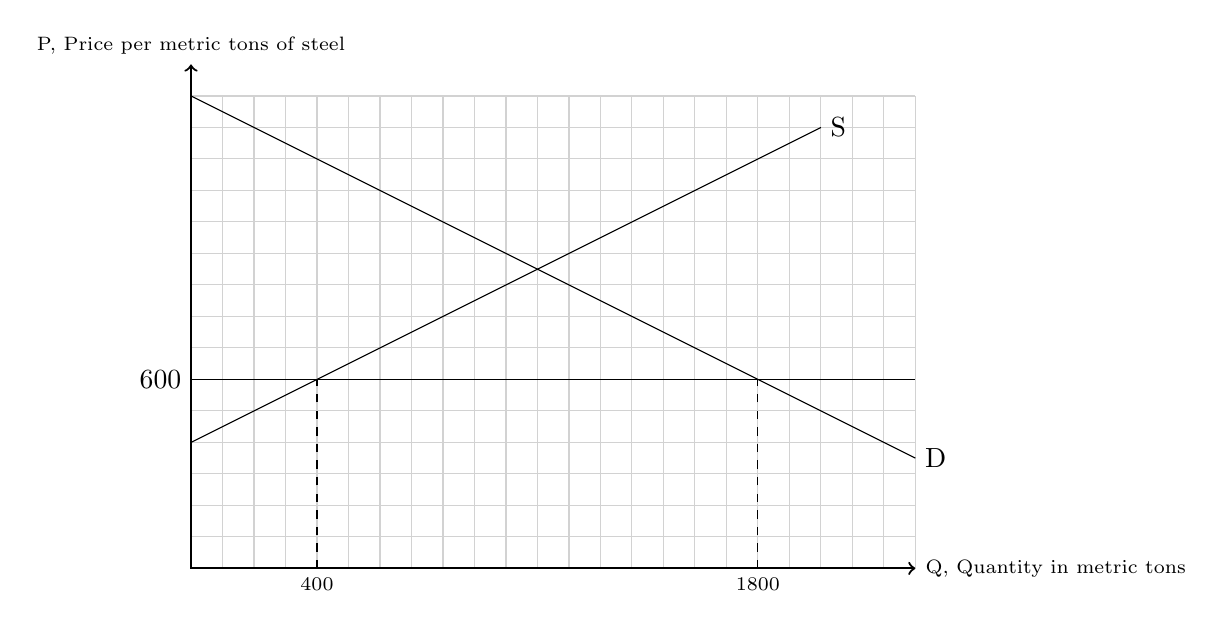
\begin{tikzpicture}[xscale=.4,yscale=.4]
			\draw [color=gray!50,opacity=0.7]  [step=10mm] (0,0) grid (23,15);
			%HOME	
			\draw[thick,<->] (0,16) node[above,font=\scriptsize]{P, Price per metric tons of steel}--(0,0)--(23,0) node[below, right,font=\scriptsize]{Q, Quantity in metric tons}; 
			\draw (0,4) -- (20,14) node[right] {S};
			\draw (0,15) -- (23,3.5) node[right] {D};
			%		\draw (0,15) -- (30,0) node[right] {D};
			\draw[] (0,6) node[left]{600} -- (23,6)  ;
			%	\draw[dashed] (0,1.8) node[left]{300} -- (1.35,1.8) -- (1.35,0) node[below,font=\scriptsize]{1.6} ;
			\draw[dashed] (4,0) node[below,font=\scriptsize]{400} -- (4,6) ;
			\draw[dashed] (18,0) node[below,font=\scriptsize]{1800} -- (18,6) ;
			%	\draw[dashed] (1,0) node[below,font=\scriptsize]{1}  ;
			%	\draw[] (0,1.5) node[left]{297} -- (2,1.5)  ;
			%	\draw[thick, red] (0,6) node[left]{$297$} -- (22,6)  ;
			%	\path[fill=yellow,opacity=0.3]	(0,.5) -- (.8,2.1) -- (0,2.1);
			%	\path[fill=blue,opacity=0.3]	(0,2.1) -- (1.2,2.1) -- (0,4.5);
			
			%	\draw[dashed]  (.8,2.1) -- (.8,-.4)  node[below,font=\scriptsize]{.62}    ;
			%	\draw[dashed]  (1.2,2.1) -- (1.2,-.4)  node[below,font=\scriptsize]{1.58}  ;
			%	\path[fill=gray,opacity=0.4]	(0.65,1.8) -- (.8,1.8) -- (0.8,2.1);
			%	\path[fill=gray,opacity=0.4]	(1.2,1.8) -- (1.2,2.1) -- (1.35,1.8);
			%	\path[fill=green,opacity=0.3] (0.8,1.5) -- (.8,2.1) -- (1.2,2.1) -- (1.2,1.5);
			%	\draw (1,1.95) node {$c_1$};
			%	\draw (1,1.65) node {$c_2$};
		\end{tikzpicture}
		%	\captionof{figure}{The effect of a tariff in a large country}\label{fig:tarlarg}
	\end{centering}	
}

\pbn
\solx{Tariff}{
		\begin{centering}
		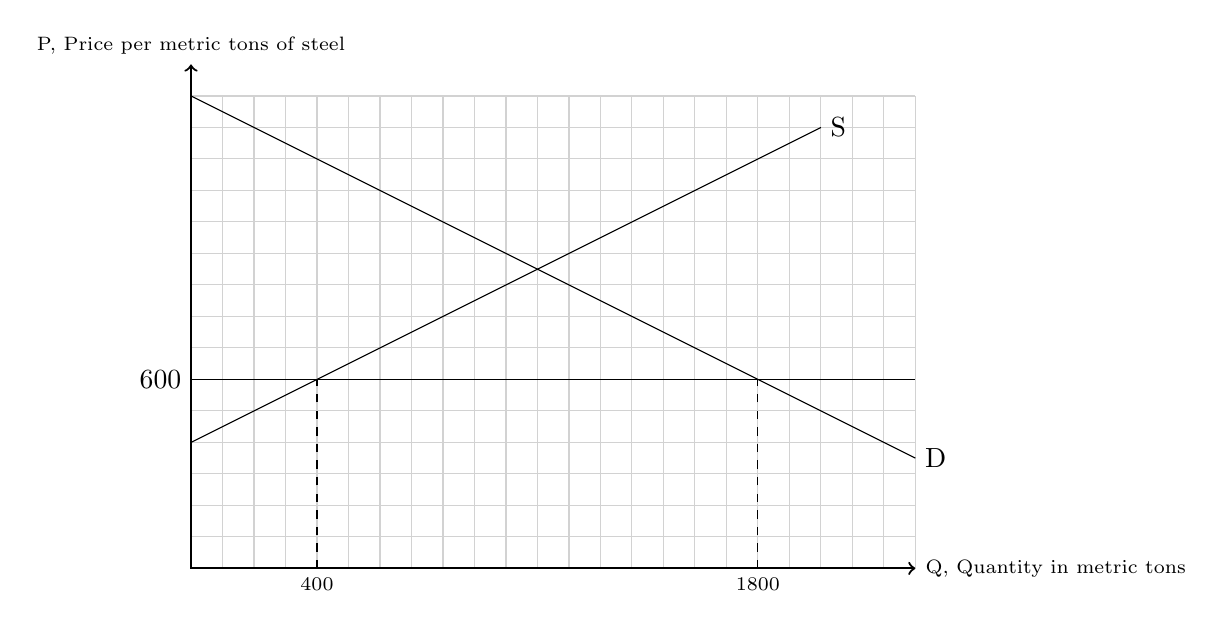
\begin{tikzpicture}[xscale=.4,yscale=.4]
			\draw [color=gray!50,opacity=0.7]  [step=10mm] (0,0) grid (23,15);
			%HOME	
			\draw[thick,<->] (0,16) node[above,font=\scriptsize]{P, Price per metric tons of steel}--(0,0)--(23,0) node[below, right,font=\scriptsize]{Q, Quantity in metric tons}; 
			\draw (0,4) -- (20,14) node[right] {S};
			\draw (0,15) -- (23,3.5) node[right] {D};
			%		\draw (0,15) -- (30,0) node[right] {D};
			\draw[] (0,6) node[left]{600} -- (23,6)  ;
			%	\draw[dashed] (0,1.8) node[left]{300} -- (1.35,1.8) -- (1.35,0) node[below,font=\scriptsize]{1.6} ;
			\draw[dashed] (4,0) node[below,font=\scriptsize]{400} -- (4,6) ;
			\draw[dashed] (18,0) node[below,font=\scriptsize]{1800} -- (18,6) ;
			%	\draw[dashed] (1,0) node[below,font=\scriptsize]{1}  ;
			%	\draw[] (0,1.5) node[left]{297} -- (2,1.5)  ;
			%	\draw[thick, red] (0,6) node[left]{$297$} -- (22,6)  ;
			%	\path[fill=yellow,opacity=0.3]	(0,.5) -- (.8,2.1) -- (0,2.1);
			%	\path[fill=blue,opacity=0.3]	(0,2.1) -- (1.2,2.1) -- (0,4.5);
			
			%	\draw[dashed]  (.8,2.1) -- (.8,-.4)  node[below,font=\scriptsize]{.62}    ;
			%	\draw[dashed]  (1.2,2.1) -- (1.2,-.4)  node[below,font=\scriptsize]{1.58}  ;
			%	\path[fill=gray,opacity=0.4]	(0.65,1.8) -- (.8,1.8) -- (0.8,2.1);
			%	\path[fill=gray,opacity=0.4]	(1.2,1.8) -- (1.2,2.1) -- (1.35,1.8);
			%	\path[fill=green,opacity=0.3] (0.8,1.5) -- (.8,2.1) -- (1.2,2.1) -- (1.2,1.5);
			%	\draw (1,1.95) node {$c_1$};
			%	\draw (1,1.65) node {$c_2$};
		\end{tikzpicture}
		%	\captionof{figure}{The effect of a tariff in a large country}\label{fig:tarlarg}
	\end{centering}	
	\enxx{(a)}{
		\item  (By analogy with \autoref{fig:tarlarg}, here we should compare the two gray triangles with area $c_2$.)
		
		The price per metric ton of steel from foreign suppliers will be \textdollar 699 because government will charge \textdollar 100 on each ton of steel which is now worth \textdollar 599 on world markets. As \textdollar 699 is still below the autarky price of \textdollar 950, domestic suppliers will set prices to be equal to \textdollar 699.  Thus,
		\begin{align*}
			699&=400+\frac{1}{2}Q^s \Leftrightarrow Q^s=598\\
			699&=1500-\frac{1}{2}Q^d \Leftrightarrow Q^d=1602\\
			1602-598&=1004
		\end{align*}
	That means, at a price of \textdollar 699 domestic supply is 598 and domestic demand is 1602 tons of steel. 1004 tons will be imported.
	
	To calculate the \textbf{welfare loss} (the two triangles), we can calculate the left triangle only and double it (please note that this is only possible if both triangles really have the same size which is only the case if both supply and demand curves have the same slope in absolute terms!):
		\begin{align*}
			\underbrace{\left(\underbrace{(598-400)}_{\text{loss in quantity}}\cdot \underbrace{\frac{1}{2}}_{\text{to get the triangle}}\cdot \underbrace{(699-600)}_{\text{increase in price}}\right)}_{\text{left triangle}}\cdot \underbrace{2}_{\text{right triangle is of same size}}=9801\cdot 2=19602
		\end{align*}
	The welfare gain (the new square that is due to the change in world market price, a.k.a. $c_2$) is $1004 [\text{tons}] \cdot  1 \left[\frac{\textdollar}{\text{tons}}\right]=\textdollar 1004.$
		Thus, overall welfare gain is 
		\begin{align*}
			1004-19602=-18598.
		\end{align*}
		That means, the welfare loss exceeds the welfare gain by \textdollar 18598.
		\item \begin{align*}
			400+\frac{1}{2}Q=1500-\frac{1}{2}Q \Leftrightarrow Q=1100\\
			P^s=400+\frac{1}{2}\cdot 1100=950
		\end{align*}
		At a price above \textdollar 950, no steel would be imported. Thus, a tariff must be so high that the price of foreign steel within the country exceeds \textdollar 950, i.e., $P^W+t>950$. Assuming that the world market price would have a lower bound of \textdollar 599, i.e., any tariff above \textdollar 100 would not decrease the world market price any further, than a tariff of (950-599=351) \textdollar 351 would make imported steel prohibitively expensive.
		\item Below a price of \textdollar 400 any domestic production would be unprofitable because the supply curve tells us that no domestic producer would be able to supply anything at and below the price of \textdollar 400. To proof that just set $Q^s=0$ in the function of the supply curve and you get $P^s=400$.
		\item At a world market price above \textdollar 950, it would be profitable to export steel because domestic supply exceeds domestic demand and the world market price is higher than the production costs.
	}
}

%
%\exex{SMOPEC with tariffs}{
%The government of a \textit{small open economy}, A,  needs your help to decide whether the introduction of a tariff of $\$20$ per unit of good $x$ is a welfare improving market intervention, or not. 
%Country A's demand and supply curves for good $x$ are given as follows:
%\begin{align*}
%	Demand: Q^d=&200-P\\
%	Supply: Q^s=&P-20.
%\end{align*}
%Moreover, you know that the world market price of good $x$ is $p^W=\$ 50$.
%
%\abcx{
%\item Draw below the world market price, as well the supply, and the demand curve of country A.
%\begin{center}
%	\begin{tikzpicture}[xscale=.5,yscale=.5]
%		\draw [color=gray!50,opacity=0.9]  [step=10mm] (0,0) grid (22,22);
%		%HOME	
%		\draw[thick,<->] (0,22) node[above,font=\scriptsize]{P, Price of  good $x$}--(0,0)--(22,0) node[below, right,font=\scriptsize]{Q, Quantity of good $x$}; 
%		\draw[] (0,5) node[left]{50};
%		\draw[] (0,10) node[left]{100};
%		\draw[] (0,15) node[left]{150};
%		\draw[] (0,20) node[left]{200};
%		\draw[] (5,0) node[below]{50};
%		\draw[] (10,0) node[below]{100};
%		\draw[] (15,0) node[below]{150};
%		\draw[] (20,0) node[below]{200};
%		%	\draw (0,2) -- (20,22) node[right] {S};
%		%	\draw (0,20) -- (20,0) node[right] {D};
%		%	\draw[] (0,5) node[left]{50} -- (22,5)  ;
%		%	\draw[] (0,7) node[left]{70} -- (22,7)  ;
%	\end{tikzpicture}
%\end{center}	
%
%
%\item What would be the price of good $x$ in the absence of trade, i.e., in autarky?
%
%\item Calculate the quantity of the country's imports under free trade.
%
%\item Calculate the government revenue of the country when it introduces a tariff of \textdollar 20.
%
%\item Calculate the value of the welfare loss and the welfare gain, respectively, that comes with the introduction of the tariff.
%
%\item  With the introduction of the tariff, do the country's consumer surplus increase, decrease, or remain equal with the introduction of the tariff?
%\item With the introduction of the tariff, do the country's producer surplus increase, decrease, or remain equal ?
%}
%}
%
%\solx{SMOPEC with tariffs}{
%\abcx{
%\item 
%\item 	\begin{center}
%	\begin{tikzpicture}[xscale=.4,yscale=.4]
%		\draw [color=gray!50,opacity=0.7]  [step=10mm] (0,0) grid (22,22);
%		%HOME	
%		\draw[thick,<->] (0,22) node[above,font=\scriptsize]{P, Price of  good $x$}--(0,0)--(22,0) node[below, right,font=\scriptsize]{Q, Quantity of good $x$}; 
%		\draw (0,2) -- (20,22) node[right] {S};
%		\draw (0,20) -- (20,0) node[right] {D};
%		\draw[] (0,5) node[left]{50} -- (22,5)  ;
%		\draw[] (0,7) node[left]{70} -- (22,7)  ;
%		\draw[] (0,5) node[left]{50};
%		\draw[] (0,10) node[left]{100};
%		\draw[] (0,15) node[left]{150};
%		\draw[] (0,20) node[left]{200};
%		\draw[] (5,0) node[below]{50};
%		\draw[] (10,0) node[below]{100};
%		\draw[] (15,0) node[below]{150};
%		\draw[] (20,0) node[below]{200};
%	\end{tikzpicture}
%\end{center}	
%
%\item 	The autarky price would be \textdollar 110.
%\item 	The quantity of the country's imports under free trade would be 120 units of good $x$.
%\item 	The government revenue of the country when it introduces a tariff of \textdollar 20 would be $\$ 20\cdot 80= \$1600$.
%\item The welfare loss would be $20\cdot \$ 20= \$400$.
%\item The consumer surplus would decrease.
%\item	The producer surplus would increase.
%}
%}

%\exex{ARTE documentary on trade wars}{Please watch the documentary on ARTE: \url{https://www.arte.tv/en/videos/087959-000-A/trade-wars/}. }



%\pbn
%\solx{Buy local be happy?}{
%	See discussion in class.
%}